

\begin{figure}[!t]
    \centering
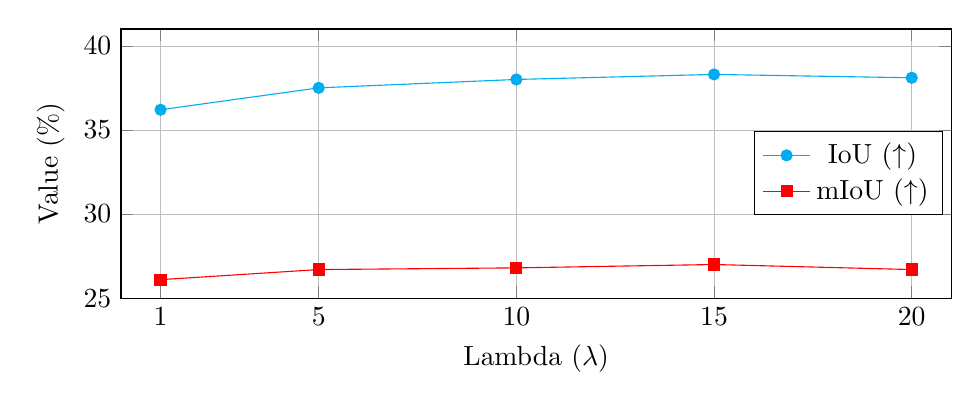
\begin{tikzpicture}
    \begin{axis}[
        width=\columnwidth,
        height=5cm,
        xlabel={Lambda ($\lambda$)},
        ylabel={Value (\%)},
        xmin=0, xmax=21,
        ymin=25, ymax=41,
        xtick={1, 5, 10, 15, 20},
        xticklabels={1, 5, 10, 15, 20},
        ytick={25, 30, 35, 40},
        legend style={at={(0.99, 0.62)}},
        grid=both,
        grid style={line width=.1pt, draw=gray!10},
        major grid style={line width=.2pt, draw=gray!50},
    ]
        \addplot[
            color=cyan,
            mark=* ,
            mark options={solid, fill=cyan},
        ] coordinates {
            (1, 36.2)
            (5, 37.5)
            (10, 38.0)
            (15, 38.3)
            (20, 38.1)
        };
        \addlegendentry{IoU ($\uparrow$)}

        \addplot[
            color=red,
            mark=square*,
            mark options={solid, fill=red},
        ] coordinates {
            (1, 26.1)
            (5, 26.7)
            (10, 26.8)
            (15, 27.0)
            (20, 26.7)
        };
        \addlegendentry{mIoU ($\uparrow$)}
    \end{axis}
\end{tikzpicture}
    \caption{\textbf{Impact of different the contribution $\lambda$ of $L_{2D}$ on 3D semantic occupancy performance.} The architecture used is TPVFormer \cite{huang2023tpv}. Models are trained using a combination of $L_{\text{2D}}$ and $L_{\text{3D}}$ with varying $\lambda$ values and evaluated on 3D IoU and mIoU. We train and evaluate the models on 20\% of Occ3D-nuScenes \cite{tian2023occ3d} training and validation datasets.}
    \label{fig:lambda_impact}
\end{figure}
